\documentclass[11pt]{book}

\usepackage[book]{header}
\usepackage[fontset = fandol]{ctex}
	% \CTEXoptions[today=old]
	% \CTEXoptions[contentsname=Table of Contents]
\usepackage{graphicx,wrapfig,paralist}
	\setlength{\pltopsep}{3pt}
	\setlength{\plpartopsep}{3pt}

\usepackage{titletoc}
	\setcounter{secnumdepth}{5}  
	\setcounter{tocdepth}{5} 

\usepackage{makeidx}
	\makeindex

\usepackage{hyperref}
	\hypersetup{bookmarksnumbered=true}

\renewcommand\thechapter{\Roman{chapter}} 

\newcommand{\rr}{\mathbb{R}}
\newcommand{\zz}{\mathbb{Z}}
\newcommand{\cc}{\mathbb{C}}
\newcommand{\aaa}{\mathfrak{a}}
\newcommand{\pp}{\mathfrak{p}}
\newcommand{\mm}{\mathfrak{m}}
\newcommand{\dd}{\mathrm{d}}
\newcommand{\oo}{\mathscr{O}}
\newcommand{\ff}{\mathscr{F}}
\newcommand{\scrg}{\mathscr{G}}
\newcommand{\scr}[1]{\mathscr{#1}}
\newcommand{\bbp}{\mathbb{P}}
\newcommand{\bba}{\mathbb{A}}
\def\A{\mathbb{A}}
\def\P{\mathbb{P}}

\DeclareMathOperator{\im}{im}
\DeclareMathOperator{\Hom}{Hom}
\DeclareMathOperator{\Mor}{Mor}
\DeclareMathOperator{\id}{id}
\DeclareMathOperator{\rank}{rank}
\DeclareMathOperator{\tr}{tr}
\DeclareMathOperator{\supp}{supp}
\DeclareMathOperator{\coker}{coker}
\DeclareMathOperator{\codim}{codim}
\DeclareMathOperator{\height}{height}
\DeclareMathOperator{\sign}{sign}
\DeclareMathOperator{\spec}{Spec}
\DeclareMathOperator{\proj}{Proj}
\DeclareMathOperator{\res}{res}

\DeclareMathOperator{\Gal}{Gal}
\DeclareMathOperator{\ann}{ann}
\DeclareMathOperator{\Ann}{Ann}
\DeclareMathOperator{\ev}{ev}

\newcommand{\hyp}{-}
\newcommand{\nottran}{\rule{2mm}{2mm}}
\newcommand{\idx}[1]{\textit{#1}\index{#1}}
\newcommand{\idxx}[2]{\textit{#2}\index{#1!#2}}

\newcommand{\moha}[1]{\stackon[1pt]{#1}{\hbox to 0pt{\hss\includegraphics[width=.8em]{naive.pdf}\hss}}}
\newcommand{\Naive}{Na\moha{\i}ve}
\newcommand{\naive}{na\moha{\i}ve}

\theoremstyle{plain}
\newtheorem{thm}{Theorem}[chapter]
\newtheorem{pro}[thm]{Proposition}
\newtheorem{lem}[thm]{Lemma}
\newtheorem{coro}[thm]{Corollary}

\theoremstyle{definition}
\newtheorem{defi}[thm]{Definition}
\newtheorem{exe}[thm]{Exercise}
\newtheorem{exa}[thm]{Example}

\renewcommand*{\proofname}{Proof}
\renewcommand{\thethm}{\thechapter\raisebox{.15ex}{-}\arabic{thm}}

\renewcommand\thechapter{\Roman{chapter}}
	\newcommand{\cc}{\mathbb{C}}

% \setCJKmainfont[
% 	ItalicFont = AdobeKaitiStd-Regular ,
% 	BoldFont = SourceHanSerifSC-Bold ,
% ]{SourceHanSerifSC-Regular}
% \renewcommand{\hyp}{\raisebox{.1em}{-}}
% \renewcommand{\textit}[1]{{\raisebox{-.1ex}{\scalebox{1.05}{\it #1}}}}

\newcommand{\picc}[1]{\begin{center}\includegraphics[scale=0.6]{#1}\end{center}}
\newcommand{\pic}[1]{\picc{#1}}
\newcommand{\ThisULCornerWallPaper}[2]{}

\begin{document}
\begin{titlepage}
\setcounter{page}{-1}
\thispagestyle{empty}
	\begin{flushright}
	{\Huge\bfseries 概形的几何}\\[\baselineskip]
	% {{\scshape In\:}\Large {\itshape a simple} {\scshape Way}} \par
	{by xxx}\par
	\today
	\end{flushright}
	\vfill
	{\Large\itshape 仅作内部交流用}
\end{titlepage}
\clearpage
\thispagestyle{empty}

\frontmatter
\tableofcontents
\mainmatter
	\chapter*{前言}
\addcontentsline{toc}{chapter}{前言}
暂略。

\vspace{2ex}

有翻译上的问题,可以选择以下方式联系译者:

\begin{itemize}
    \item QQ:{\tt 2236211567}
    \item Github: \url{https://github.com/chaoli-math/197}
    \item email: {\tt 2236211567@qq.com}
\end{itemize}

本翻译仅供消遣娱乐。
	\def\PICDIR{chap_1/pics}

\chapter{基本定义}\label{chap:1}
\ThisULCornerWallPaper{1}{Pictures/1.png}
\renewcommand{\pic}[1]{\picc{chap_1/pics/#1}}

\chapter{基本定义}
\section{仿射概形}

\subsection{作为集合的概形}
\section{一般的概形}
\section{相对概形}\index{相对!概形}
\subsection{纤维积} \label{s.1.3.1}

这里有一个用概形的纤维积描述的,集合关于函数的原像思想的重要拓展。为了准备这个定义,我们首先复习集合范畴的情况。

两个集合$X$和$Y$在第三个集合$S$上的纤维积,在已知一个映射的图
\[
	\xymatrix{
	&X\ar[d]^\varphi\\
	Y\ar[r]_\psi &S
	}
\]
下,被定义为
\[
	X\times_S Y=\{(x,y)\in X\times Y\,:\,\varphi x=\psi y\}.
\]
纤维积有时候被叫做$X$(或者关于$X\to S$)到$Y$的\textit{拉回}\index{拉回}。这个构造以一种非常有用的方式拓展了许多基础构造:

如果$S$是一个点,则它给出了一般的直积。

如果$X$和$Y$都是$S$的子集,而$\varphi$和$\psi$都是含入映射,则它给出交。

如果$Y\subset S$以及$\psi$是含入,他给出了$Y$在$X$中的原像。

如果$X=Y$,他给出了使得$\varphi$, $\psi$相等的集合,即映射的\textit{等值子}。

\begin{exe}
	验证这些断言!
\end{exe}

注意到,$X\times_S Y$与它到$X$和$Y$自然的投射给出了交换图
\[
	\xymatrix{
	X\times_S Y\ar[r]\ar[d]&X\ar[d]^\varphi\\
	Y\ar[r]_\psi &S
	}
\]
实际上,集合$X\times_S Y$能被下面的泛性质所确定:在所有使得下图交换的$Z$与给定的映射下
\[
	\xymatrix{
	Z\ar[r]\ar[d]&X\ar[d]^\varphi\\
	Y\ar[r]_\psi &S
	}
\]
$X\times_S Y$与投射是唯一的“最有效的”选择,意即,给定上图中的$Z$,存在唯一的映射$Z\to X\times_S Y$使得图
\[
	\xymatrix{
	Z\ar[dr]\ar[ddr]\ar[drr] & &\\
	& X\times_S Y \ar[r]\ar[d] &  X \ar[d]^\varphi\\
	& Y\ar[r]^\psi &  S
	}
\]
交换。

在概形范畴中,我们就\textit{定义}纤维积是一个满足上面泛性质的概形,特别地,泛性质保证了这个概形连同他到$X$和$Y$的投射是唯一的。于是我们能用纤维积来定义直积、交、原像以及等值子!但这就有一个问题,是否作为纤维积的这些对象在概形范畴是存在的?答案是是的,我们下面将描述它的构造。

首先,我们处理仿射情形。回忆仿射概形范畴与交换环范畴对偶,见Corollary \ref{coro:1.41}. 因此,如果我们有概形
\[
	X=\spec A,\quad Y=\spec B,\quad S=\spec R,
\]
其中$X$, $Y$映到$S$(因此$A$和$B$是$R$\hyp 代数),我们必须定义纤维积$X\times_S Y$为
\[
	X\times_S Y=\spec(A\otimes_R B).
\]
这是因为自然的图
\[
	\xymatrix{
	A\otimes_R B&A\ar[l]\\
	B\ar[u]&R\ar[l]\ar[u]_\varphi
	}
\]
有着与纤维积相反的泛性质。时髦一点说法即,张量积即一个交换环范畴的\textit{纤维余积}或者\textit{纤维直和}。

为了检查这个定义是合理的,可以注意到当$Y$是$S$的由$I$定义的闭子概形,即$B=R/I$时,我们有$A\otimes_R B=A/IA$. 于是$X\times_S Y=\spec A/IA$,这就是以前定义过的$Y$在$X$中的原像。

\begin{exe}\label{exe:1.46}
一些简单的特殊例子将在计算纤维积的时候给出巨大的帮助。直接通过代数的张量积的泛性质证明下面的事实:

\begin{compactenum}[(a)]
\item 对任意的$R$\hyp 代数$S$,我们有$R\otimes_R S=S$.
\item 若$S$, $T$是$R$\hyp 代数,$I\subset S$是一个理想,于是
\[
	(S/I)\otimes_R T=(S\otimes_R T)/(I\otimes 1)(S\otimes_R T).
\]
\item 如果$x_1$, $\dots$, $x_n$, $y_1$, $\dots$, $y_m$是不定元,于是
\[
	R[\text{$x_1$, $\dots$, $x_n$}]\otimes R[\text{$y_1$, $\dots$, $y_m$}]=R[\text{$x_1$, $\dots$, $x_n$, $y_1$, $\dots$, $y_m$}].
\]
\end{compactenum}
用这些原理来解决习题的剩余部分。
\begin{compactenum}[(a)] \setcounter{enumi}{3}
\item 令$m$, $n$是整数。计算纤维积
\[
	\spec \zz/(m)\times_{\spec \zz} \spec \zz/(n).
\]
\item 计算纤维积$\spec \cc \times_{\spec \rr} \spec \cc$.
\item 证明,对$R$上的任意多项式环$R[x]$和$R[y]$,我们有
\[
	\spec R[x]\times_{\spec R}\spec R[y]=\spec R[x,y].
\]
\end{compactenum}
注意在例子(d)中,纤维积的支集是两个对应支集的纤维积,但是这在(e)和(f)中并不正确。
\begin{compactenum}[(a)] \setcounter{enumi}{6}
\item 考虑环同态
\[
	R[x]\to R;\quad x\mapsto 0
\]
以及
\[
	R[x]\to R[y];\quad x\mapsto y^2.
\]
证明关于这些映射,我们有
\[
	\spec R[y]\times_{\spec R[x]}\spec R=\spec R[y]/(y^2).
\]
\end{compactenum}
\end{exe}

在一般的情况中,我们用仿射概形$\spec R_\rho$来覆盖$S$,以及将它们在$X$和$Y$中的原像相应用仿射概形$\spec A_{\rho\alpha}$和$\spec B_{\rho\beta}$来覆盖,于是我们可以说
\[
	\xymatrix{
	&X\ar[d]^\varphi\\
	Y\ar[r]_\psi &S
	}
\]
被如下形式的图
\[
	\xymatrix{
	&\spec A_{\rho\alpha}\ar[d]^{\varphi_{\rho\alpha}}\\
	\spec B_{\rho\beta}\ar[r]_{\psi\beta} &\spec R_{\rho}
	}
\]
所覆盖。

当然,我们已经知道最后一幅图中的纤维积是$\spec(A_{\rho\alpha}\otimes_{R_\rho}B_{\rho\beta})$. 使用在上节末段提供的粘合思想,虽繁但不难验证这些概形在相交处相容,并且粘合起来就得到了所需的概形$X\times_S Y$,我们略去这些计算。纤维积的另一个构造方法将在第\ref{s:5.2.1}节中略加提到。

马上,我们就可以用纤维积来给出在仿射概形$S$上的仿射空间$\bba_S^n$的另一种描述:

\begin{exe}\label{exe:1.47}
令$S$是任意概形。令$\bba_\zz^n=\spec \zz[x_1$, $\dots$, $x_n]$是在$\spec \zz$上的仿射空间,之前已经定义过它了(这个概形将在下一章详细描述)。证明,$S$上的仿射空间$\bba_S^n$能被描述为纤维积:$\bba_S^n=\bba_\zz^n\times_{\spec \zz} S$.
\end{exe}

我们同样能用纤维积来定义一个态射$\psi:Y\to X$在任意概形的任意点上的\textit{纤维}:如果$p$是一个$X$的点对应于$R$的素理想$\pp$,则$\psi$在点$p$处的纤维是$Y$与单点的概形$\spec \kappa(p)$的纤维积。当$X$和$Y$都是仿射概形时,记$Y=\spec T$以及$X=\spec R$,作为点集,我们有
\[
	\psi^{-1}(p)=\spec \kappa(p)\times_X Y=\spec (R_\pp /\pp_\pp \otimes_R T)=\spec (R_\pp/\pp_\pp \otimes_R T/\pp T).
\]
这是$T$中所有原像在$R$中等于$\pp$的素理想的集合。更一般地,定义一个$X$的闭子概形$X'$关于态射$\psi$的\textit{原像}或者称为\textit{逆像}为纤维积$X'\times_X Y$.

就像在上面处理的仿射情况中那样,$X'$的原像$\psi^{-1}X'$是一个$Y$的闭子概形。使用$\oo_Y$上的$\oo_X$\hyp 结构,原像的理想层可以写作$\mathscr{I}_{\psi^{-1} X'}=\mathscr{I}_{X'}\cdot \oo_Y$.

另一个使用纤维积的典型范例是在研究簇在基域扩张下的表现(某些人常常在某些上下文中称为“基变换”而不是纤维积)。我们将在下面的章节中看到这个背景中的不少例子,概形理论的这个概念为处理算术问题提供了足够的自由与便利。

\nottran

\subsection{\texorpdfstring{$S$}{S}\hyp 概形范畴}

就像在集合范畴里面一样,我们能用纤维积得到绝对积,通过取$S$为概形范畴的终对象,终对象即一个概形$S$使得每一个概形都有到$S$唯一的态射。由Exercise \ref{exe:1.42},概形范畴的终对象是$\spec \zz$. 然而,绝对积有着许多更加惊奇的性质。我们已经在Exercise \ref{exe:1.46}(d) 中看到,(当$m$和$n$互素时)两个非空集合的积可能是空的!概形的积同样还有其他奇怪的特性:比如,一个不可约概形的维度能被定义为其任意仿射开集的坐标环的Krull维度。我们可能希望两个概形的积
\[
	X\times Y=X\times_{\spec \zz} Y
\]
的维度是$X$和$Y$的维度的和。但实际上,我们有下题中的结论。

\begin{exe}\label{exe:1.48}
证明,如果$X=\spec \zz[x]$以及$Y=\spec \zz[y]$,那么
\[
	\dim X\times Y=\dim X+\dim Y-\dim \spec \zz=\dim X+\dim Y-1.
\]
\end{exe}

\begin{exe}\label{exe:1.49}
令$K$是一个域。如果$X$和$Y$是非空$K$\hyp 概形,于是在$K$\hyp 概形范畴,积$X\times Y=X\times_{\spec K}Y$是非空的。
\end{exe}
\section{点函子}

概形的一个有趣地方是它们有着许多并不能由拓扑空间所表达的结构,所以那些集合上的熟悉操作,比如取直积,此时就需要警惕地审查,以免它们在概形上没有意义。 但值得注意的是,许多集合论式的想法可以通过点函子
\footnote{译者注:没找到靠谱的翻译,先这样翻着。}
(the functor of points)这个简单的技术来应用到概形上。虽然这个观点一开始为问题增加了一层复杂性,但它是富于启发性的,因此,点函子以及相关术语的应用相当普遍。我们将在这里简要介绍必要的定义,后面的章节会偶尔使用它们,直至第 \ref{chap:6} 章会详细介绍。

从一个观察开始,概形的点一般来说并不相似:我们有非闭点和闭点;如果我们在非代数闭域上工作,那么即使是闭点也可以通过它们不同的剩余类域来区分。类似地,如果我们在$\mathbb{Z}$上工作,不同点可能具有不同特征的剩余类域;如果我们把点的概念扩展到“底空间只有一点的闭子概形”,我们甚至会有更大的多样性。 而且当然地,概形之间的态射根本不由其底空间之间的映射决定。

然而,存在一种观察概形的方法,它将观察约化到集合上,它就是概形的点函子。更准确地说,我们可能将一个概形看作一族集合,一个概形范畴上的函子,在上面集合中那些熟悉的操作依然成立%
%\footnote{译者吐槽:这样啥都不说,然后藏着掩着说一些特性,读着真是让人摸不着头脑。个人建议,读这本书先把定义看了,然后再反过头看前面的引入,作者爷爷把定义的许多解释先摆出来了。嗯,再或者,似乎可以假设大家都精通这些定义。}%
。在本节中,我们将研究如何用函子来描述概形。这样做的一个巨大回报是,我们能将概形范畴嵌入到一个更大的函子范畴中,在那里许多构造将变得更简单。这样做的好处很类似于,在分析中,我们考虑分布而不是普通的函数%
%\footnote{译者注:说的 是广义函数那一套,大家都懂的。}
。它把在概形范畴的如何进行构造的问题转移到了理解哪些函子来自于概形。此外,许多概形范畴中的几何构造能以一种有用的方式拓展到更大的函子范畴中。

为了引入点函子的概念,我们从一般的范畴理论开始。首先,在那些对象是具有附加结构的集合的范畴,对象$X$的集合$|X|$能用从一个泛对象到$X$的态射集描述;比如:
\begin{compactenum}[(a)]
\item 在可微流形范畴,如果$Z$是只包含一个点的流形,则对于任意的流形$X$,我们有$|X|=\Hom(Z,X)$.
\item 在群范畴,对任意的群$X$我们有$|X|=\Hom(\zz,X)$.
\item 在同态都将单位元映作单位元的含幺环范畴,如果我们令$Z=\zz[x]$,则对任意的含幺环$X$,我们有$|X|=\Hom(Z,X)$.
\end{compactenum}

一般地,对范畴$\mathscr{X}$中的任意对象$Z$,对应
\[
	X\mapsto \Hom_{\mathscr{X}}(Z,X)
\]
定义了一个从范畴$\mathscr{X}$到集合范畴的函子。正如前面第一段所说的,然而,把集合$\varepsilon(X)= \Hom_{\mathscr{X}}(Z,X)$叫做对象$X$的点的集合并不是令人满意的,除非这个函子是\textit{忠实的},即除非对$\mathscr X$的任意两个对象$X_1$和$X_2$,态射
\[
	f:X_1\to X_2
\]
由集合之间的映射
\[
	f':\Hom_{\mathscr{X}}(Z,X_1)\to \Hom_{\mathscr{X}}(Z,X_1)
\]
所决定。

这个条件不是总能满足的。比方说,令$\text{(Hot)}$是$CW$-复形的范畴,其中$\Hom_\text{(Hot)}(X,Z)$是$X$到$Z$之间连续函数的同伦类集合。如果$Z$是一个单点复形,则
\[
	\Hom_\text{(Hot)}(X,Z)=\pi_0(X)
\]
是$X$的连通分支的集合,所以这并不能给出一个忠实函子。而且,我们也不可能选一个更好的对象$Z$. 同样,在概形范畴,没有对象$Z$能干这种事。

为修正这点,Grothendieck机智地选择同时考虑全部的集合$\mathrm{Mor}(Z,X)$而不仅是其中一个!即,我们对每一个概形$X$,给定一个“结构化集合”,它包含了所有的集合$\mathrm{Mor}(Z,X)$,同时,对每一个态射$f:Z\to Z'$,通过复合$f$给出了映射$\mathrm{Mor}(Z',X)\to \mathrm{Mor}(Z,X)$.

用更形式化地语言来说,概形$X$的\textit{点函子}是由$X$决定的“可表”函子,即,函子
\[
	h_X:(\text{schemes})^\circ\to (\text{sets}),
\]
其中$(\text{schemes})^\circ$和$(\text{sets})$分别表示箭头反过来的概形范畴以及集合范畴。$h_X$将每一个概形$Y$变成集合
\[
	h_X(Y)=\mathrm{Mor}(Y,X)
\]
以及每一个态射$f:Y\to Z$变成集合的映射
\[
	h_X(Z)\to h_X(Y)
\]
通过将$g\in h_X(Z)=\mathrm{Mor}(Z,X)$变成复合$g\circ f\in \mathrm{Mor}(Y,X)$. “可表函子”的名字来自于这个函子被一个概形$X$所\textit{表示}。集合$h_X(Y)$被称为$X$的\textit{$Y$-值点}的集合(如果$Y=\spec T$是仿射的,我们经常用$h_X(T)$来代替$h_X(\spec T)$,并且称其为$X$的$T$-值点的集合)。

再引入一层抽象,注意到这定义了一个函子
\[
	h:(\text{scheme})\to \text{Fun}((\text{scheme})^\circ,(\text{sets}))
\]
(其中函子范畴的态射是自然变换),满足
\[
	X\mapsto h_X
\]
以及对每一个态射$f:X\to X'$给出了一个自然变换$h_X\to h_{X'}$,即对任意的概形$Y$,将$g\in h_X(Y)=\mathrm{Mor}(Y,X)$变成了复合$f\circ g\in h_{X'}(Y)=\mathrm{Mor}(Y,X')$.

当然,当我们操作$S$-概形的时候,我们也应只考虑$S$-概形态射。这种情况完全类似上面的情况:我们这样描述了一个函子
\[
	X\mapsto h_X,
\]
它从$S$-概形范畴到范畴
\[
	 \text{Fun}((\text{$S$-scheme})^\circ,(\text{sets})).
\]

这种看着抽象的想法根植于对方程组解的研究。令$X=\spec R$是一个仿射概形,其中$R=\zz[x_1$, $x_2$, $\dots]/(f_1$, $f_2$, $\dots)$. 如果$T$是任意其他环(可以将$T$想做$\zz$, $\zz/(p)$, $\zz_{(p)}$, $\hat \zz_{(p)}$, $\mathbb{Q}_p$, $\rr$, $\cc$等),一个从$\spec T$到$\spec R$的态射等价于一个从$R$到$T$的环同态,它将由$x_i$的像$a_i$所确定。当然,一族元素$a_i\in T$在这种方式下确定了一个态射,当且仅当,它们是方程组$f_i=0$的解。综上,我们已展示了
\[
	h_X(T)=\left\{
		\parbox{11em}{
			那些是方程组$f_i=0$的解的$T$中的点列$a_1$, $\dots$
		}
	\right\}.
\]

类似地,如果$X$是任意概形,于是$X$是一族仿射概形$X_a$的并,这些仿射概形相交于开集,于是从一个仿射概形$Y$到$X$的态射可以通过给出$Y$的一个基本仿射开覆盖$Y_{f_a}$以及从$Y_{f_a}$到$X_a$的映射来描述,这些态射在相交的开集上相同(一些$Y_{f_a}$当然可能是空的)。

于是,$h_X(Y)$中的一个元素依然可以在一个更广义的上下文中理解为一族方程的解,关联于一些$X_a$,在 \nottran

即使有了上面的解释,点函子的概念看上去还是略显乏味:尽管可以用这种新的语言来表述问题,但我们是否可以用它来解决问题还不甚明晰。我们可以在这套语言下工作的关键在于,许多概形范畴的显然的几何概念能被自然地拓展到更大的函子范畴中。比如,我们可以讨论一个函子的开子函子、闭子函子,光滑函子,一个函子的切空间等等。这些概念将在第 \ref{chap:6} 章展开,在那里我们同样会给出如何使用它们的一个更好理解。

在这章中,我们以两种方式用过“点”这个词:一是概形$X$的点,二是对任意概形$Y$,$X$的$Y$-值点的集合。千万不要混淆这两种用法,因为它们是非常不同的概念:比如,如果$Y=\spec L$,其中$L$是$\mathbb{Q}$的一个有限扩张,于是我们有映射
\[
	\{\textit{$X$的$Y$-值点}\}\to |X|,
\]
但这个一般来说既不是单的也不是满的:它的像是$X$中剩余类域$\kappa(p)$是$L$的子域的那些$p$的集合,以及,在这样的一个点处的纤维是一族从$\kappa(p)$到$L$的环同态。另一个差别是,$|X|$中的点是绝对的,但是$X$的$Y$-值点的集合是相对的,它可能依赖于基概形$S$以及结构态射$X\to S$. 最后,当$S=\spec K$时,$X$的$K$-值点的集合,即那些满足$\kappa(p)=K$的$p\in X$的集合,经常被叫做$X$的\textit{$K$-有理点}。

这两种“点”的概形都具有一些(但不是全部)我们期望的集合范畴中点的性质。比方说,积$X_1\times X_2$的$Y$-值点的集合就是$X_1$和$X_2$的$Y$-值点集合的积。然而,对并$X=U\cup V$的$Y$-值点的集合,此时并不是$U$, $V$的$Y$-值点集合的并(比方说,恒等映射$X\to X$是$X$的一个$X$-值点,但一般来说它并不包含于$U$或者$V$中)。相较之下,对概形$X$的点的集合$|X|$,上面的论断成立。

现在,我们已经列出了概形理论的基本定义。下一章中,我们将给出许多例子,从这些例子身上,读者将得到概形的一些“直观与感受”。
	\def\PICDIR{chap_2/pics}

\chapter{例子}\label{chap:2}
\ThisULCornerWallPaper{1}{Pictures/2.png}
\section{代数闭域上的约态概形}

概形概念的发始,即是想要推广经典的代数闭域上的仿射簇,我们将从它开始一系列关于概形的例子。在这里,代数闭域$K$上的仿射簇是指一个仿射概形$\spec R$,其中$R$是一个簇$X$的坐标环\index{坐标环},即$R$是一个有限生成的约态$K$\hyp 代数\index{约态!代数}。(回忆一个环是约态的,是指它没有非零幂零元。)$\spec R$时常被叫做\textit{相伴于簇}$X$的概形\footnote{译者注:在下面的行文中,翻译中也会将$\spec R$称为$X$的相伴概形。同时,有时候也会反过来,称一个簇或者闭点相伴于某个概形。由于有时候一个理想也给出一个簇,所以有时也会用相伴于理想的概形,或者理想的相伴概形等说法。}:这种概形有时就直接被称作仿射簇。在以后几节中,我们将考虑不同于这个基本模型的概形。

相伴于代数闭域$K$上的仿射簇的$K$\hyp 概形与这个簇是等价的对象:它们都可以决定一个相同的坐标环或者被一个相同的坐标环决定。但是,在这个例子中已经有所表现的是,在概形理论中,一些经典的概念,比如簇的相交或者映射的纤维,应有更精确的解释。在这以及接下来的章节中,我们将看到这个现象的例子。

\subsection{仿射空间}

我们从概形$\mathbb{A}^n_K:=\spec K[x_1$, $\dots$, $x_n]$开始,其中$K$是一个代数闭域。这个概形被称为$K$上的\textit{仿射}$n$-\textit{空间}。

这里将使用一个标准但绝不平凡的代数结论 ------ Hilbert's Nullstellensatz(零点定理)的一种形式;比如可见 Eisenbud [1995].

\begin{thm}[Nullstellensatz]
	设$K$是一个域,如果$\mathfrak{m}$是多项式环$K[x_1$, $\dots$, $x_n]$的一个极大理想(或者更一般地,$p$是$K$上的一个代数空间的子簇的一个闭点),则
	\[
		K[x_1, \dots, x_n]/\mathfrak{m}=\kappa(p)
	\]
	是一个有限维$K$\hyp 矢量空间。
\end{thm}

在我们的例子中,$K$是代数闭的,这就意味着$\kappa(p)=K$. 因此,记$\lambda_i$是$x_i$在$\kappa(p)$中的像,可以看到
\[
	\mathfrak{m}=(x_1-\lambda_1, \dots, x_n-\lambda_n).
\]
于是,$\mathbb{A}^n_K$中的闭点与$K$中元素的$n$元组相对应,正如期望的那般。有时,我们会用“点$(\lambda_1$, $\dots$, $\lambda_n)$”来指代“点$[(x_1-\lambda_1$, $\dots$, $x_n-\lambda_n)]$”. 

从一维的情况开始,仿射直线
\[
	\mathbb{A}^1_K=\spec K[x]
\]
长得就像它的经典对应,同样被叫做仿射直线的仿射簇。在仿射直线上,每一个$\lambda\in K$都对应有一个闭点,闭点构成的集合上的Zariski拓扑也与仿射簇上的经典的Zariski拓扑相同:开集是有限集的补。概形$\mathbb{A}^1_K$与簇不同的地方只在于它多了一个点,这个点被称为\textit{一般点}\index{一般!点}%
\footnote{译者注:作者后面才会给出明确的定义,这里事先给一下:如果$Y=\overline{\{x\}}$,则称$x$是$Y$的一个一般点。一般而言,一般点可能不存在,也可能不唯一。}%
,对应于零理想$(0)$。
\vspace{-1ex}\inclugra{1.png}\vspace{-2ex}
点$(0)$的闭包是整个$\mathbb{A}^1_K$,因此,$\mathbb{A}^1_K$的闭子集就是$\mathbb{A}^1_K-\{(0)\}$的有限子集。

仿射平面$\mathbb{A}^2_K=\spec K[x,y]$同样与它的经典对应相似,但现在就多了许多点,同时也表现得更加有趣。像之前一样,我们有来自于极大理想$(x-\lambda,y-\mu)$的闭点,对应于寻常平面中的$(\lambda,\mu)$. 但现在却有两类非闭点。首先,对每一个不可约多项式$f(x,y)\in K[x,y]$,有一点$p$对应于素理想$(f)\subset K[x,y]$,它的闭包包含$p$本身以及所有使得$f(\lambda,\mu)=0$的闭点$(\lambda,\mu)$,点$(f)$被称为该集合的一般点。一般地,概形中的每一个点都被称为该点闭包的一般点。比起簇$\mathbb{A}^2_K$,在概形$\mathbb{A}^2_K$中,对每一条不可约平面曲线,我们都需要加入一点,这个点属于这条曲线的闭包,且该点的闭包等于曲线的闭包。最后,正如在$\mathbb{A}^1_K$中,我们还需加入一个对应于零理想的点,即$\mathbb{A}^2_K$的一般点,它的闭包是整个$\mathbb{A}^2_K$.

\inclugra{2.png}

因为$K[x,y]=K[x]\otimes_K K[y]$,从定义有
\[
	\mathbb{A}^2_K=\mathbb{A}^1_K\times_{\spec K}\mathbb{A}^1_K.
\]
在这里,纤维积显然是一个正确的积,但它作为集合并不等于其因子作为集合的积。

仿射空间$\mathbb{A}^n_K$是上一个例子的直接推广:几何上,可以看到概形$\mathbb{A}^n_K$是经典的仿射$n$-空间对每一个正维数的不可约子簇$\Sigma$加上一点$p_\Sigma$. 与前面一样,$p_\Sigma$属于$\Sigma$的闭包中,且$p_\Sigma$的闭包等于$\Sigma$的闭包,是$\Sigma$的一般点。

更一般的,设$X\subset \mathbb{A}^n_K$是任意的仿射簇,对应于理想$I\subset \mathbb{A}^n_K$以及坐标环$R=K[x_1$, $\dots$, $x_n]/I$,我们能得到对应的仿射概形$\spec R$,并可以通过商映射$K[x_1$, $\dots$, $x_n]\to R$将它看作$\mathbb{A}^n_K$的一个子概形。这个概形,与$\mathbb{A}^n_K$的情形类似,长得就像仿射簇$X$但还需要对每一个正维数的不可约子簇$\Sigma\subset X$加入一个新的一般点$p_\Sigma$.

纤维,或者更一般的原像,是除了簇之外,概形最有可能出现在经典代数几何中的方式。

\begin{exe} \label{exe:2.2}
设$\varphi:K[x]\to K[x]$是一个环同态,他将$x$变成$x^2$,考虑$\varphi$诱导的$\spec K[x]$到自身的映射。证明,在概形意义上,点$0$的纤维是由$(x^2)$定义的子概形。

\inclugra{3.png}
\end{exe}

在所有的概形中,代数闭域上仿射簇的相伴概形被如下性质的环$R$的谱所刻划,
\begin{compactitem}[~~~--]
\item 有限生成
\item 约态代数\index{约态!代数}
\item 在一个域上
\item 这个域是代数闭域
\end{compactitem}

为了对更一般的概形长什么样有所感觉,以及对它们有什么益处有所把握,我们在接下来的几节中考虑撤去上面四条限制中的几条后将会发生什么。我们会主要考虑那些上面四条限制中只有一条不满足的情况,因为理解它们将帮助我们理解更一般的情况;在习题中,偶尔会提到更复杂的例子。

\subsection{局部概形}

我们的第一类不同于簇的概形的例子是局部环的谱,称之为\textit{局部概形}\index{局部!概形}。我们这里将考虑的例子是代数闭域上约态代数的谱,但不一定是有限生成的。局部概形常常作为技术性工具来研究其他更几何的概形:它们经常被用来关注仿射概形的局部结构上。在只有一个闭点的例子中,概形比起簇新增的点将变得更加醒目。自然,只用一个几何点来表示这些概形是错误的,取而代之的,它们应当被看成簇的芽。只有一个闭点的现象不是新近才被代数学家研究的,作为类似物,当考虑复解析流形上一点处的芽时它已经出现了,那里它给出了一点$x$处“足够小”的邻域的图像:比如,在这个“足够小”的邻域中,每条经过$x$的曲线都可以被区分开来,尽管它们可能除了$x$之外再无在任意的邻域中有定义的点。在局部环的谱上,我们将看到类似的图像。

首先考虑环$K[x]$关于极大理想$(x)$的局部化$K[x]_{(x)}$,令$X=\spec K[x]_{(x)}$. 空间$|X|$只有两个点:一个闭点对应于极大理想$(x)$,另一个开点对应于零理想$(0)$,他的闭包包含点$(x)$. 含入同态$K[x]\hookrightarrow K[x]_{(x)}$诱导了一个映射$X\to \mathbb{A}_K^1$,于是我们将$X$看作$\mathbb{A}_K^1$的子概形(尽管$|X|$在$\mathbb{A}_K^1$不是开的也不是闭的)。子概形$X$是“局部的”,因为$X$是所有$\mathbb{A}_K^1$中包含$(x)$的开集的交%
\footnote{译者注:若一个拓扑空间存在一般点,则其任意开子集都包含所有的一般点。设$\mathbb{A}_K^1$中所有包含$(x)$的开集的交为$U$,因此$X=\{(0),(x)\}\subset U$. 反过来,对任意闭点$p\in \mathbb{A}_K^1$,则$\mathbb{A}_K^1-p$是一个包含$(x)$的开集,但是并不包含$p$,所以$p\not\in U$. 于是$X=U$. 这个命题可以如下推广:设$X$是一个拓扑空间,对$x\in X$,记所有$x$的开邻域的交为$S_x$,则$S_x=\{y\,:\, x\in \overline{\{y\}}\}$.}%
,于是,比如,$X$上的正则函数正好就是$\mathbb{A}_K^1$上在点$0=(x)$处正则的有理函数,即它们是$\mathscr{O}_{\mathbb{A}_K^1}(U)$中的元素,其中$U$是$\mathbb{A}_K^1$中包含点$0=(x)$的某个邻域。在这层意味上,$X$是$\mathbb{A}_K^1$在原点处的芽。

接着,考虑概形$X=\spec R$,其中$R=K[x,y]_{(x,y)}$是$K[x,y]$关于极大理想$(x,y)$的局部化,极大理想$(x,y)$对应于点$(0,0)$. 同上,我们有映射$X\to \mathbb{A}_K^2$,这里我们能将$X$看成$\mathbb{A}_K^2$中所有$(0,0)$的邻域的交。类似地,$X$只有一个闭点,但现在却有了无穷多的非闭点,每一个都对应于一条经过原点的不可约曲线。于是,$X$的子概形是$\mathbb{A}_K^2$的子概形在$(0,0)$的芽,以及$X$本身是$\mathbb{A}_K^2$在$(0,0)$的芽。

对$\mathbb{A}_K^n$乃至对$\mathbb{A}_K^n$的每一个子概形,都有类似的构造:如果$X=\spec K[x_1,$ $\dots$, $x_n]/I\subset \mathbb{A}_K^n$是一个理想为$I$的仿射簇的相伴概形,而$\mathfrak{m}$对应于$X$的一个闭点,我们能将概形$\spec K[x_1,$ $\dots$, $x_n]_\mathfrak{m}/I_{\mathfrak{m}}$看成$X$中$[\mathfrak{m}]$的一个邻域的芽。与在许多语境中谈论一个空间上一点处的函数芽不同,在概形理论中,芽依然是一个概形。

在某些场合,这样引入的局部概形实际上还不够局部:概形一点处的局部环依然包含着许多概形整体结构的信息。比如,非奇异簇$X$的概形在不同闭点处的芽不一定是同构的,尽管当我们考虑由同一个方程定义的复解析簇$X^{\text{an}}$时,任意两点的芽确实是同构的。出现这个现象的实质在于这里用来定义芽的开集太大了。为了在概形语境下得到一个更局部的图像,我们需要观察幂级数环对应的概形:比如,比起考察$\mathbb{A}_K^2$处原点$(0,0)$某个邻域的芽$X=\spec K[x,y]_{(x,y)}$,我们转而考虑概形$Y=\spec K [\![x,y]\!]$. 与前面的例子类似,它只有一个闭点$[(x,y)]$以及一个一般点$[(0)]$,一般点的闭包是整个$Y$,此外,对每一个$x$和$y$的不可约幂级数$\sum a_{i,j}x^iy^j$,$Y$上都对应着有一点。映射 %proofread
\[
	K[x,y]\hookrightarrow K[x,y]_{(x,y)}\hookrightarrow K[\![x,y]\!]
\]
给出了映射$Y\to X\to \mathbb{A}_K^2$,于是我们能把$Y$想象成比$X$“更小的”原点的邻域。(然而,注意到$X$和$Y$都不是$\mathbb{A}_K^2$的开子概形或闭子概形。)比如,如果$X$中对应于素理想$(y^2-x^3-x^2)$的曲线是不可约,且域$K$的特征不是$2$,则$\mathbb{A}_K^2$中被这个方程定义的曲线在$Y$中的原像是两个(非平凡)曲线的并。因为$x^2+x^3$有着幂级数表示的平方根
\[
	u=x+\frac{1}{2}x^2-\frac{1}{8}x^3+\cdots.
\]
因此我们能把$y^2-x^3-x^2$分解为
\[
	y^2-x^3-x^2=(y-u)(y+u),
\]
所以概形$\spec  K[\![x,y]\!]/(y^2-x^3-x^2)$是可约的。(见下图。)

\inclugra{4.png}

当然,为使这样的事是可行的,$Y$必然比$X$有“更多”曲线,下面的习题补充了这点。

\begin{exe}
	\begin{compactenum}[(a)]
		\item 同上,设$u=\sqrt{x^2+x^3}$,那么$[(y-u)]$在$\spec K[x,y]$中的像是什么?(提示:这是一个包含$y^2-x^3-x^2$的素理想。)
		\item 证明,$Y$中的点$(y-\sum_{n\geq 1}x^n/n!)$在$\mathbb{A}_K^2$中的像是$\mathbb{A}_K^2$的一般点。
	\end{compactenum}
\end{exe}

一般地,在上面的映射$Y\to X$下,一点的原像对应于一条$\mathbb{A}_K^2$的不可约曲线$C$,它由原点处$C$的所有解析分支构成。(更多关于分支的讨论见Walker [1950]或者Brieskorn以及Kn\"{o}rrer [1986].)

虽然这里有了局部概形的另一个重要例子,但上面的概形$Y$的一个问题是,Exercise {\theexe}(b)中的点与代数的观点相去甚远。为了避免这点,我们可以转而考虑幂级数环的子环$H\subset K[\![x,y]\!]$的谱$Z$,其中环$H$在$K[x,y]$的分式域$K(x,y)$上满足一个代数方程。我们称其为概形$X$的\idx{Hensel化},概形$Z$居于$Y$与$X$之间,使得我们有一列映射
\[
	Y\to Z\to X\to \mathbb{A}_K^2.
\]
这种构造的用处在于,$H$是一系列有限生成$K$\hyp 代数的并,于是$Z$是一族概形的逆极限,这族概形每一个都来自于寻常的簇。几何上来看,$Z$是在$\mathbb{A}_K^2$在\textit{\'{e}tale拓扑}\index{\'{e}tale!拓扑}下的芽。这个概念我们这里按下不表,详细可见Artin [1971].

\begin{exe}
	当$K=\mathbb{C}$,如何将收敛幂级数构成的环的谱纳入这种图像中?
\end{exe}
\section{非代数闭域上的约态概形}

我们现在考虑当观察非代数闭域上的有限生成约态代数的谱时将会发生什么。对这样的结构的兴趣最开始来自于数论,当然,他远比概形理论要早得多!比如,关于有理二次型的研究,数论中一个古老的课题,能看作对有理数域上二次方程定义的簇的研究。研究有理数域上三个变量的三次型在数论上至今依然是非常活跃的方向,其中现在主要醉心于$\mathbb{Q}$上的椭圆曲线理论。最基本的对象是$\mathbb{Q}$上的代数簇(或是$\mathbb{Z}$上的概形,我们以后会回到这个情况),但是在处理它们的过程中,数论学家常常使用下面这副图中这些所有的基环,以及许多的中间域以及中间环:
\[
\begin{xy}
	\xymatrix{
		\hat{\mathbb{Z}}_{(p)}\ar[r]&\hat{\mathbb{Q}}_{p}\ar[rr]&&\mathbb{C}_p\\
		\mathbb{Z}_{(p)}\ar[u]&&&\\
		\mathbb{Z}\ar[u]\ar[r]\ar[d]&\mathbb{Q}\ar[r]\ar[uu]&\mathbb{R}\ar[r]&\mathbb{C}\ar[uu]\\
		\mathbb{F}_p\ar[r]&\bar{\mathbb{F}}_p&&&
	}
\end{xy}
\]
概形理论提供了一个相当富有弹性且舒适的框架来处理这些基环的改变。同时,一个性质良好的约态簇,在模$p$后可能突然变成一个非约态的东西,描述这东西需要更完整的概形理论(比如见2.4.4节)。

从最简单的例子开始,考虑$\mathbb{A}_{\mathbb{R}}^1=\spec \mathbb{R}[x]$. 使用Nullstellensatz,我们能看到$R[x]$中有两类极大理想:一种的剩余类域是$\mathbb{R}$,它们具有形式$(x-\lambda)$,其中$\lambda\in\mathbb{R}$,剩余类域是$\mathbb{C}$,它们具有形式$(x+\mu x+\nu)$,其中$\mu$, $\nu\in\mathbb{R}$且满足$\mu^2-4\nu<0$. 第二类理想可以写作$((x-z)(x-\bar{z}))$的形式,其中$z\in \mathbb{C}$不是一个实数。于是,$\mathbb{A}_{\mathbb{R}}^1$中的闭点,对应于一个实数或者一对共轭的复数。最后,$\mathbb{A}_{\mathbb{R}}^1$同样有着唯一的非闭点,他对应于素理想$(0)$,它的闭包是整个$\mathbb{A}_{\mathbb{R}}^1$.

接着,我们来到$\mathbb{R}$上的仿射平面,$\mathbb{A}_{\mathbb{R}}^2=\spec \mathbb{R}[x,y]$,以及考虑$R[x,y]$的极大理想$\mathfrak{m}$给出的闭点。同样从Nullstellensatz,$R[x,y]$关于$\mathfrak{m}$的剩余类域只有$\mathbb{R}$与$\mathbb{C}$,于是复合映射
\[
	\rr\to \rr[x,y]/\mm\cong (\rr \text{ or } \cc)
\]
或者是恒同或者是$\rr$到$\cc$的含入。取$\lambda$和$\mu$作为$x$和$y$在$\cc$中的像,对前一种情况,我们可以看到$\mm=(x-\lambda,y-\mu)$对应于$\rr^2$中一般意义上的点。但是对后一种情况,$\mm$同时对应于$(\lambda,\mu)$和$(\bar\lambda,\bar\mu)$:从另一种视角来看,将$x$, $y$变成$\lambda$, $\mu$的同态$\rr[x,y]\to \cc$与另一个将$x$, $y$变成$\bar\lambda$, $\bar\mu$的同态有着相同的核,因为它们只差一个$\cc$在$\rr$上的自同构。

给出上面描述的极大理想的生成元并不是件很困难的事情。如果$\rr[x,y]/\mm\cong \rr $,很清楚地,$\mm=(x-\lambda,y-\mu)$. 另一方面,假设$\lambda$是实数,则$\mu$必须要满足一个不可约二次实系数多项式$y^2+ay+b=0$,于是$\mm$包含理想$(x-\lambda,y^2+ay+b)$. 但是这个理想显然是一个素理想(比如,先提出$x-\lambda$因子),于是$\mm=(x-\lambda,y^2+ay+b)$. 自然,当$\mu$是实数的时候,类似的结果也成立。

最后,假设$\mu$和$\lambda$都不是实数,于是$\mm$包含以$\mu$和$\lambda$为根的不可约实系数多项式$f$和$g$,但是,因为$g$可以在$\rr/(f(x))\cong \cc$上分解为
\[
	g(u)=(y-\mu)(y-\bar\mu),
\]
因此$(f(x),g(y))$不是素理想!在复数域上,可以给出如下图像:

\pic{5.png}

于是$f(x)=0$与$g(y)=0$决定的轨迹是两条水平线与数值线的并,反之亦然,它们相交于四点$(\lambda,\mu)$, $(\bar\lambda,\mu)$, $(\lambda,\bar\mu)$和$(\bar\lambda,\bar\mu)$. 多项式
\[
	h(x,y)=\mathrm{Im}(\mu) x - \mathrm{Im}(\lambda)  y -\mathrm{Im}(\mu\bar\lambda)
\]
是连接$(\lambda,\mu)$和$(\bar\lambda,\bar\mu)$的那条实系数直线。理想
\[
	(f(x),h(x,y))=(g(y),h(x,y))\subset \rr[x,y]
\]
严格包含理想$(f(x),g(y))$中,这个理想就是我们寻找的极大理想,这点可以通过检查
\[
	\rr[x]\cong \rr[x,y]/(h)\cong \rr[y]
\]
得到(这些同构中,注意到$(\bar\mu-\mu)$与$(\bar\lambda-\lambda)$都非零)。
\section{非约态概形}

我们现在离开那些能被看作概形的对象,即那些仿射概形$\spec R$而$R$是有一个有限生成代数闭域上的代数,且没有幂零元。这里的现象将变得不再那么熟悉,我们需要在他们身上花费更多努力。

这类概形在一些足够简单的几何背景下就已经出现了:比如,下面处理的多重点已经作为两个寻常概形的相交或者作为映射“退化的”纤维出现了,正如Exercise \ref{exe.2.2}中看到的。另一类非约态概形重要的应用在一族簇的理论(theory of families of varieties):形变理论(deformation theory)以及模理论(moduli theory)。我们将解释如何对一族单参数的簇取极限,以及引入关键概念,平坦性。最后,我们将给出一些非约态概形的例子,就它们自身而言都是有趣的对象。

从最简单的情况入手,我们将关注仿射空间$\mathbb{A}_K^n$的子概形,其支撑包含原点 ------ 等价地,它由一个理想$I$给出,其零点集$V(I)$作为集合包含$(0$, $\cdots$, $0)$. (回忆一个概形的支撑是指它自有的那个拓扑空间。)

\subsection{双重点}

\begin{exa}
	此类概形最简单的例子是$\mathbb{A}_K^1$由理想$(x^2)$定义的子概形 ------ 即概形$\spec K[x]/(x^2)$,通过商映射$K[x]\to K[x]/(x^2)$诱导的映射看作$\mathbb{A}_K^1$的子概形。这个概形只有一个点,对应于理想$(x)$,
\end{exa}

\subsection{多重点}

\subsubsection*{度与重数}
\addcontentsline{toc}{subsubsection}{度与重数}

\subsection{嵌入点}

\subsubsection*{准素分解}
\addcontentsline{toc}{subsubsection}{准素分解}

\subsection{概形的平坦族}

\subsubsection*{极限}
\addcontentsline{toc}{subsubsection}{极限}

\subsubsection*{例子}
\addcontentsline{toc}{subsubsection}{例子}

\subsubsection*{平坦性}
\addcontentsline{toc}{subsubsection}{平坦性}

\subsection{多重直线}
\section{算数概形}

我们最后一类概形是有限生成约态环但不包含任意域的环的谱。一般地,有限生成$\zz$-代数的谱被称为\textit{算术概形}\index{概形!算术},它们主要在数论中出现,尽管并非所有数论学家感兴趣的概形都具有这种形式。在这些例子中,我们将看到概形在算术以及几何的观点之间的惊人统一的许多线索。\nottran

\subsection{$\spec \mathbb{Z}$}

我们从最明显的例子开始,概形$\spec \zz$. 环$\zz$的素理想当然是$(p)$,其中$p$是素数,以及$(0)$,前者对应于$\spec \zz$的闭点,剩余类域是$\mathbb{F}_p$,后者是一个“一般”点,闭包是整个$\spec \zz$而剩余类域是$\mathbb{Q}$. 图像如下:

% \pic{15.png}

\noindent 这与域上的直线$\mathbb{A}_K^1$在形式上是相似的,事实上,这只是一系列类比的开始,因此在看下面的例子时应将其铭记在心。然而,这种类比也有着它的不足:尽管$\spec \zz$表现得很像$\mathbb{A}_K^1$,但比如$\mathbb{A}_K^1$是$\mathbb{P}_K^1$的稠密开子概形,而$\spec \zz$不是任何一个概形的稠密开子概形。

\subsection{数域中整数环的谱}

其次,考虑概形$\spec A$,其中$A\subset K$是数域$K$中的整数环。作为例子,我们将分析$K=\mathbb{Q}[\sqrt{3}]$以及$A=\mathbb{Z}[\sqrt{3}]$. 正如$\spec \zz$的情况,$\spec A$有两类点,一类对应于$A$的非零素理想,具有有限剩余类域,另一类是一个一般点,对应于$(0)$,剩余类域是$K$. 含入映射$\zz\hookrightarrow A$诱导的映射$\spec A\to \spec \zz$让这个例子变得有趣起来。比如说,考虑点$[(p)]\in \spec \zz$处的纤维,这就是$A$中包含理想$pA\subset A$的所有素理想的集合,他将表现为下面三种方式中的一个(关于这里没解释的材料的一个好的基础参考文献是Serre [1979]):

\begin{enumerate}[{(1)}]\setlength{\itemsep}{0pt}
	\item 如果$p$整除$K$在$\mathbb{Q}$上的判别式$12$,即对$p=2$或$3$,理想$(p)$是$A$中一个理想的平方,我们有
	\[
	2A=(1+\sqrt{3})^2
	\]
	以及,当然,
	\[
	3A=(\sqrt{3})^2.
	\]
	点$(1+\sqrt{3})$和点$(\sqrt{3})\in\spec A$的剩余类环分别为$\mathbb{F}_2$和$\mathbb{F}_3$.

	\item 否则,如果$3$是一个模$p$的二次剩余,于是素理想$(p)$能分解为两个不同素理想的乘积,比如
	\[
	11A=(4+3\sqrt{3})(4-3\sqrt{3})
	\]
	以及
	\[
	13A=(4+\sqrt{3})(4-\sqrt{3}).
	\]
	在这些点的剩余类域依然是元素个数为素数的有限域,分别是$\mathbb{F}_{11}$以及$\mathbb{F}_{13}$.

	\item 最后,如果$p>3$以及$3$不再是一个模$p$的二次剩余,比如$p=5$或者$7$时,理想$pA$依然是素理想,它对应于$\spec A$中的一个点。在这种情况下,剩余类域是$\mathbb{F}_p$的二次扩张,比如在上面的两个例子中是$\mathbb{F}_{25}$以及$\mathbb{F}_{49}$.
\end{enumerate}

一般地,,如果$K$是一个二次数域,$A$是$K$中的代数整数环,那么包含$Z\subset A$诱导了概形的映射$\psi:\spec A\to \spec \zz$,$\psi$在每一个闭点$(p)\in \spec \zz$处的纤维是下面的可能中的一个:

\begin{enumerate}[{(1)}]\setlength{\itemsep}{0pt}
	\item 一个非约态的点,其坐标环同构于$A/\pp^2$. 他在$\spec \zz$中的像是约态点$\pp$,而剩余类域是$\mathbb{F}_p$,如果$p$在$A$中\textit{分岔},即$pA$是$A$中一个素理想$\pp$的平方。

	\item 两个约态点$\pp$和$\pp'$的并,剩余类域是$A/\pp=A/\pp'=\mathbb{F}_p$,如果$pA$是$A$中两个不同素理想的乘积。

	\item 一个约态点,它的剩余类域$A/\pp$是$\mathbb{F}_p$的二次扩张,如果$p$在$A$中仍然是素的。
\end{enumerate}

在每个粒子中,纤维的坐标环作为$\mathbb{F}_p$-代数,维数都是2. 这是因为$A$是一个秩为2的自由$\zz$-模。这里感兴趣的类比是,映射$\spec A\to \spec \zz$与Riemann面的一个分支覆盖(或者更一般地,一个代数闭域,比如$\cc$上的一维概形)。 基本上,我们能将$\spec A$想象成$\spec \zz$的两层覆盖然后在“分岔”素数上分支,比如就像,$\spec \cc[z]$是$\spec \cc[z^2]$的一个双重覆盖,它在原点处分支。对于$\spec \zz$处的点,一个明显的不同是,分岔点处我们有两个不同的重数为1的点,但在不同于分岔点的点$(p)\in \spec \zz$处,我们只有一个重数为1的点,其剩余类域是$\mathbb{F}_p$的二次扩张,这样的点在下图中我们以均匀的灰色点表示:

% \pic{16.png}

% \subsection{$\spec \mathbb{Z}$上的仿射空间}
% \subsection{$\spec \mathbb{Z}$上的锥}
% \subsection{$\mathbb{A}_K^1$中的双重点}
	% \renewcommand{\pic}[1]{\picc{chap_3/pics/#1}}

\chapter{射影概形}
\ThisULCornerWallPaper{1}{Pictures/3.png}

在我们理解了仿射概形后,射影概形\index{射影!概形}的理论并不会包含太多新奇的东西:在大多数情况下,它与射影簇的经典理论的差别完全类似于仿射概形和仿射簇的经典理论之间的差别。

我们首先将引入两个有限性条件,\textit{有限}以及\textit{有限型},然后定义和讨论\textit{分离}以及\textit{逆紧}态射\index{逆紧!态射},它们分别对应于绝大多数几何中的Hausdorff性与紧性。而正是部分因为射影簇和概形有这些性质,它们才是经典代数几何以及概形理论的基本研究对象。

这章的下一部分将引入射影概形以及给出一些例子。如同仿射概形的情形,有两种入手射影概形的法子:一种是定义出射影空间然后取它们的子概形,另一种是将所有的射影概形建立在同一个根基上,从分次代数入手。正如处理仿射情况那般,这里我们采用第二种方法。

在介绍了射影概形的基础定义以及它们的子概形后,我们将描述射影概形之间的态射,相较于仿射对应,它将更加微妙而难以捉摸(就像在簇范畴中那样)。我们将用一些射影概形的例子结束这节,其中最值得注意的是Grassmannian.

本章的最后一节将给出嵌入在射影空间中的射影概形的三个不变量,它们由 David Hilbert 所引入:Hilbert 多项式、Hilbert 函数以及自由分解(free resolution). 使用它们,我们有时能区分类似的概形,比如射影双重直线,以及可以
揭示平坦性的一些新现象。在一个射影概形的不变量中,可以根据其 Hilbert 多项式定义的不变量的是它的度数;在这方面的联系,我们将讨论著名的 B\'{e}zout 定理。

\section{一些态射的性质}\label{s:3.1}

\subsection{有限性条件}\label{s:3.1.1}

在大多数有关概形的非平凡结论中,有两个有限性条件。它们有着相似的名字但非常不同的性质。第一个有限性条件,有限型,是一个在绝大多数几何背景中产生的态射都满足的直截了当的性质,他被引入常是为了排除无穷维的纤维或者“非几何”的概形,比如局部环的谱。而另一个有限性条件,有限,比较起来就是一个非常严格的条件:它是说一个态射是逆紧的以及它的所有纤维都是有限的(特别地,零维的)。

首先,我们称一个概形间的态射$\varphi:X\to Y$是\textit{有限型}的,如果对每一点$y\in Y$,都存在一个$y$的仿射开邻域$V=\spec B\subset Y$使得它的原像被一族仿射开集$U_i\cong \spec A_i$有限覆盖,即
\[
	\varphi^{-1}(V)=\bigcup_{i=1}^n U_i,
\]
并且在映射
\[
	\varphi_V^\#:B=\oo_Y(V)\to \oo_X (\varphi^{-1}V)\to \oo_X(U_i)=A_i
\]
下,每个$A_i$都是一个有限生成$B$\hyp 代数。因此,比如,任意$\mathbb{A}_K^n$或$\mathbb{P}_K^n$的子概形是在$K$上有限型的(意思是,结构态射$X\to \spec K$是有限型的),而一个正维数的局部$K$\hyp 代数的谱不是。

一个态射$\varphi:X\to Y$被称为\textit{有限}\index{有限}的,如果对每点$y\in Y$都有它的一个开仿射邻域$V=\spec B\subset Y$使得原像$\varphi^{-1}(V)=\spec A$也是仿射的,以及通过拉回
\[
	\varphi_V^\#: B =\oo_Y(V)\to \oo_X(\varphi^{-1}V)=A,
\]
$A$是一个有限生成$B$-模。这是一个比有限型更强的条件,首先,马上可以由其给出$\varphi$的纤维是有限的,其次,拓扑空间之间的映射$|\varphi|:|X|\to |Y|$是一个闭映射。因此,对$Y=\spec B$以及多项式$f\in B[x]$,如果$f$的最高项系数是一个可逆元但其他不是,则态射$\spec(B[x]/(f))\to Y$是有限的。这些都可以参考 Eisenbud [1995, Chapter 4 and Section 9.1].

\subsection{逆紧性和分离性}\label{s:3.1.2}

许多几何技术当应用于紧Hausdorff空间时可以获得最完整的结果。尽管仿射概形在Zariski拓扑下是预紧的,但是它们并不共享在其他理论中紧空间的良好属性,因为Zariski拓扑不是Hausdorff的。举个例子,即使$X$是预紧的,仿射概形间的正则映射$\varphi:X\to Y$的像也可能不是闭的。

Zariski拓扑并不Hausdorff这点还有着其他令人不爽的结果。回忆在流形的一般定义中,我们从一个Hausdorff空间开始,在它上面装备一个坐标卡的覆盖,坐标卡是一个标准型(即欧式空间中的球)。但注意到,即使这些球都是Hausdorff的,也不足以说明整个空间是Hausdorff的。这就是为什么在Exercise \ref{exe:1.44} 中描述的具有双重原点的直线(这里重新展示如下)

\begin{center}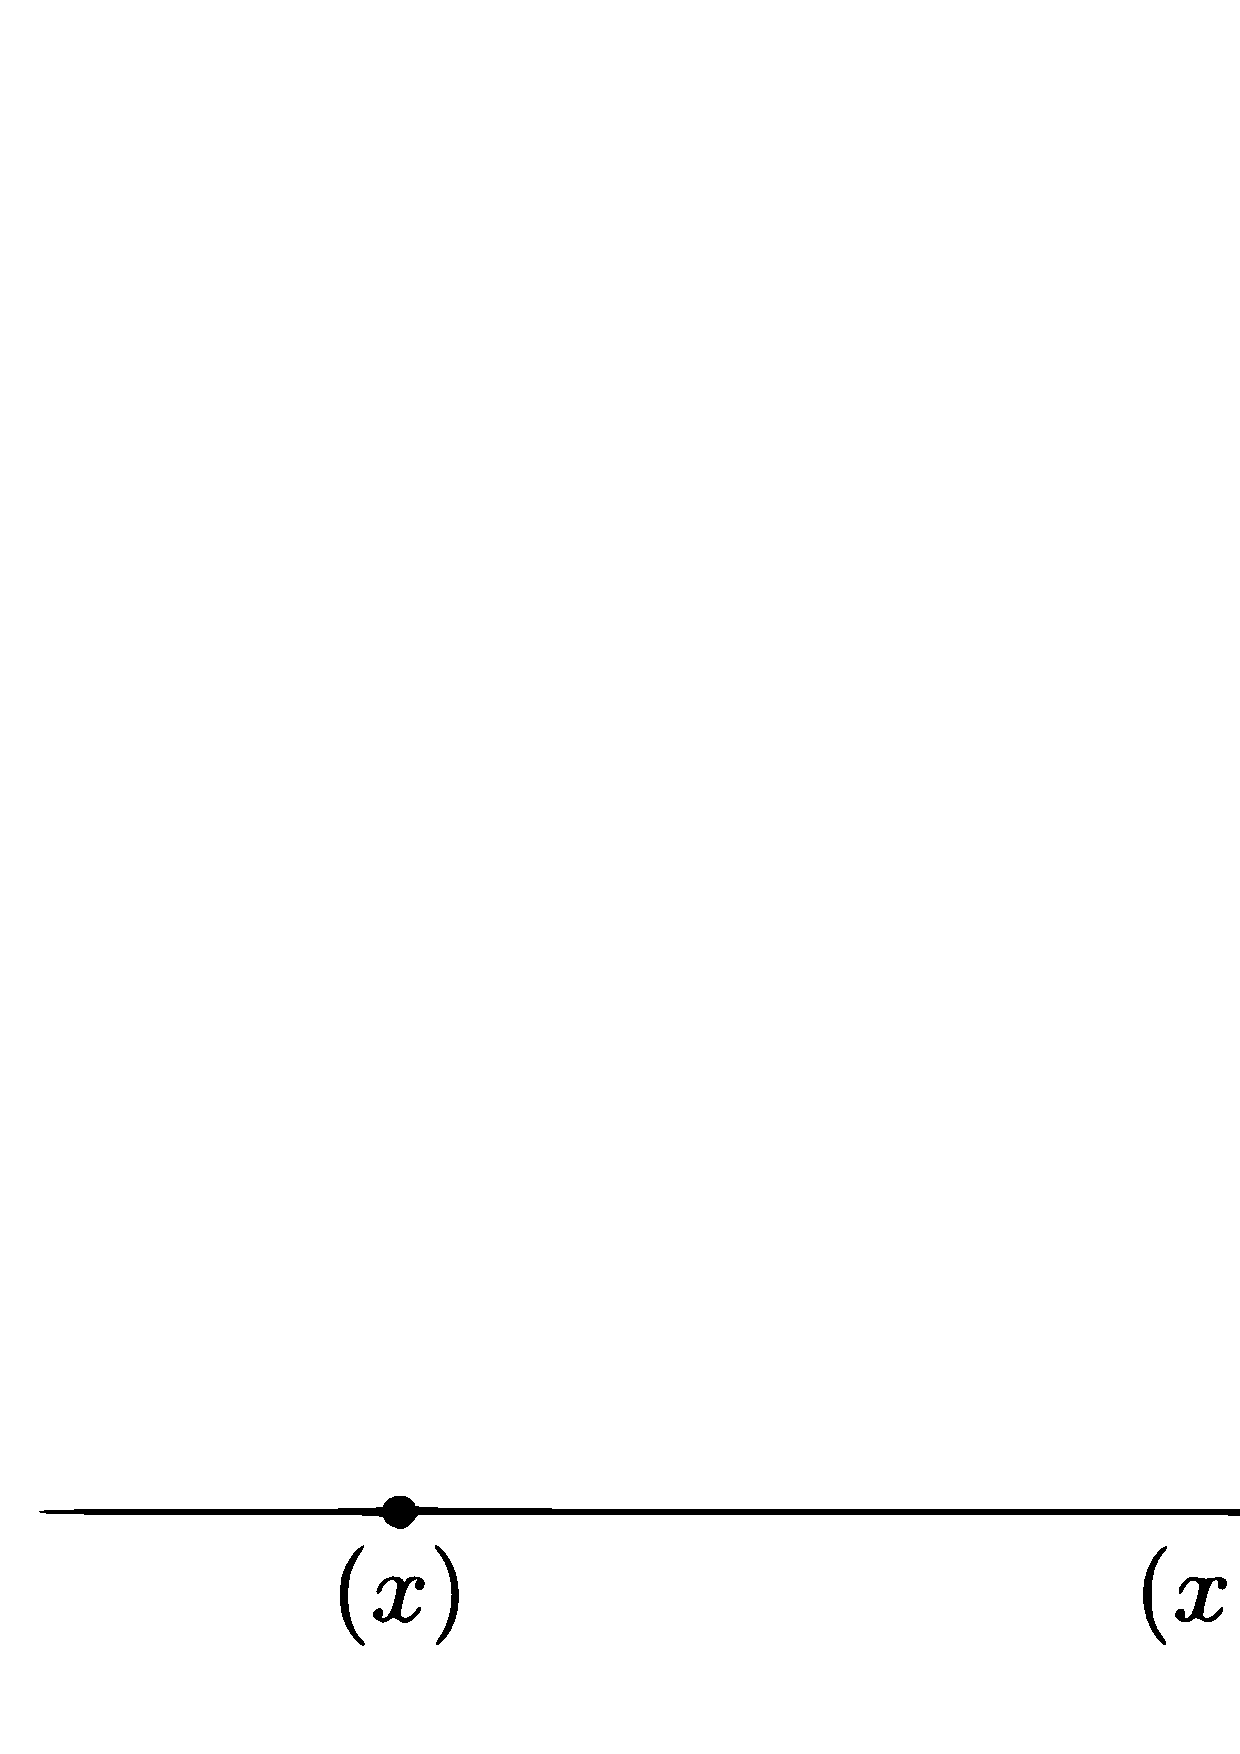
\includegraphics[scale=\scale,bb=0 0 562 68]{\PICDIR/1.png}\end{center}

\vspace{-0.4em}\noindent 不是一个流形。然而,在处理由仿射概形拼成的概形(或者簇)的时候,我们不能指定整个空间是Hausdorff的,因为即使就局部来说,那些拼合部件也不是Hausdorff的。于是,对给定两个概形之间的两个态射$\varphi$, $\psi:X\to Y$,$\varphi$和$\psi$相等的点构成的集可能不会是闭的。下面的习题是这方面的一个典型例子。

\begin{exe}
\begin{compactenum}[(a)]
\item 令$Y$是在域$K$上的具有双重原点的直线,正如在Exercise \ref{exe:1.44} 中的定义,以及令$\varphi_1$, $\varphi_2:\mathbb{A}_K^1\to Y$是两个显然的含入映射,证明$\varphi_1$和$\varphi_2$相等的点(仅作为拓扑空间间的连续映射)构成的集合不是闭的。
\item 现在令$X=Y\times_K Y$以及$\varphi$和$\psi$分别是两个到$X$到$Y$的典范投射。证明,$\varphi$和$\psi$相等的点构成的集合不是闭的(注意到这就是下面要定义的对角线)。证明,使得$\varphi$和$\psi$相等的闭点构成的集合也不是闭的。所以,这个病态现象并不是概形特有的,它在簇范畴中已经出现了。
\end{compactenum}
\end{exe}

然而,当$X$是一个仿射概形时,这样的病态现象并不会出现,同样,当$X$是一个射影概形时,这样的事情也被证明是不会出现的。这些概形所具有的理想性质,正是对应的流形上Hausdorff性的最重要结果之一(分离性),它表为:$X$作为一个概形在$K$上是\textit{分离的}。一般地,给定概形间的任意的映射$\alpha:X\to S$,我们定义\textit{对角}子概形$\Delta\subset X\times_S X$如下:局部地,在$X\times_S X$的每一个仿射开集上
\[
	X\supset \spec A\xrightarrow{\alpha|_{\spec A}}\spec B\subset S,
\]
它由所有形如
\[
a\otimes 1 - 1\otimes a \in A\otimes_B A
\]
的元素生成的理想$I$所定义。接着,我们称$\alpha$是\textit{分离的},或者说$X$是\textit{在$S$上分离的概形},如果$\Delta$是$X\times_S X$的一个闭子概形。

\begin{exe}
令$Y\to S$是拓扑空间之间的一个映射,然后令
\[
	\Delta \subset Y\times_S Y
\]
是其对角。证明,如果$\Delta$是一个闭集,那么对任意的交换图
\[
	\xymatrix{
		X\ar@<0.3ex>[rr]^\varphi \ar@<-0.3ex>[rr]_\psi\ar[dr] &&Y\ar[ld]\\
		&S&
	}
\]
$X$中使得$\varphi$和$\psi$相等的点集是一个闭集。现在证明对概形正则映射的相似引理:证明,存在一个自然定义的(即,极大的)闭子概形使得限制在上面$\varphi$和$\psi$是相同的。
\end{exe}

\begin{exe}
	令$X$是一个在$S$上分离的概形。证明$X$的(闭或开)子概形依然在$S$上分离。
\end{exe}

\begin{exe}
	注意,从对角子概形的定义来看,仿射态射是分离的。
\end{exe}

我们在下面将看到射影概形(等等就会定义)同样是分离的,因此,至少这些Hausdorff空间的性质对它们也是成立的。

在经典的仿射簇的情形中(即使简单如平面曲线),在上个世纪初就意识到,得到一些表现得像一个紧的对象的东西(实际上,在复数域上的仿射簇的情形中,在通常的拓扑下就是紧的),最简单的方式是取一个仿射簇在射影空间中的闭包。事实证明,如果$\varphi:X\to Y$是一个射影簇之间的映射,那么$\varphi$确实会将$X$的闭子簇映成$Y$的闭子簇。稍一般些,如果我们取这样一个映射以及一个任意的簇$Z$,得到
\[
	\psi:=\varphi\times 1_Z:X\times Z\to Y\times Z,
\]
则$\psi$将$X\times Z$的闭子簇映到$Y\times Z$的闭子簇。事实证明,\textit{这个性质连同分离性是使得射影概形如此有用的核心性质}。但是,满足这性质的簇要比射影簇稍多,而且它有时比起射影性更容易验证,所以给一个更一般的定义很重要。

如果$\alpha:X\to S$是一个概形之间的有限型映射,如果$\alpha$是可分的且对所有的映射$T\to S$,纤维积的投影
\[
	X\times_S T\to T
\]
将闭子集变成闭子集,则称$\alpha$是\textit{逆紧的},或者说$X$\textit{在$S$上逆紧}。同前,如果$S=\spec R$是一个环,我们时常会说“在$R$上逆紧”来意指“在$\spec R$上逆紧”。

上面对$\alpha$在分离性外给出的条件时常被叫做$\alpha$是\textit{全景闭的}。\textit{逆紧}这个名字来自一个旧的几何概念:一个Hausdorff空间之间的映射$\alpha:M\to N$被称为逆紧的如果每一个紧集的原像都是紧的。这是映射$\alpha$的一种相对紧性。这个性质与我们的定义之间的联系见下面的习题。

\begin{exe}
令$\mathscr C$是具有可数拓扑基的局部紧Hausdorff空间构成的范畴。证明映射$f:X\to Y$在$\mathscr C$中是全景闭的当且仅当他是逆紧的,即对任意的$Y$中的紧集$C$,$f^{-1}(C)$也是紧的。
\end{exe}

不管对于概形还是对于簇,逆紧这个概念已被证明是代数几何中的关键性质,它起到了其他几何理论中“紧且Hausdorff”的作用。下面我们将引入的射影概形是最一般的在给定概形$B$上逆紧的概形的例子。我们这里不会证明这个关键的结论,它并不是很难,但是将把我们引开太远。证明可以参见,比如,Hartshrone [1977, Theorem II.4.9].

一个有限态射$\varphi:X\to Y$当然是逆紧的,见Eisenbud [1995, Section 4.4].

\section{分次环的\texorpdfstring{$\proj$}{Proj}}

\subsection{\texorpdfstring{$\proj S$}{Proj S}的构造}

\subsection{\texorpdfstring{$\proj R$}{Proj R}的闭子概形}
\section{射影概形的不变量}\label{s:3.3}

在本节中,我们假设$K$是一个域,并且只在$K$-概形上工作,
除非明确提及相反的情况。

假设给定了射影空间中的一个概形,我们如何找到它的不变量?
最简单的想法是问:有多少独立的$d$-次形式在上面为零?
将对不同的$d$的答案放在一起,我们得到了以前被称为概形的假设
的东西(可能是因为当时人们对这些数给定的概形感兴趣)。 
现在,通常以等效形式的Hilbert函数来讨论这些信息。
我们将在这里讨论Hilbert函数方法的几种变体,
这些变体产生了一大类不变量。有些生成的不变量实际上
仅依赖于抽象概形,而不依赖于给定的射影嵌入,而其他的不变量则
依赖于嵌入; 所以我们将一路评注这些事情。我们采用的思路 % p.125
就是最初Hilbert [1890]使用的,而不是更被广为采用Samuel的
(比如可见Hartshorne [1977, Chapter I])。 Hilbert的方法
要求稍多一些的技巧但是能给出一个更强且更易理解的结果。

我们从定义基本的不变量开始。在这章的最后部分,我们将展示
一些简单的几何示例,说明不变量包含哪些信息。

\subsection{Hilbert函数与Hilbert多项式}\label{s:3.3.1}

首先,假设我们给定了一个闭子概形$X\subset \mathbb P^r_K$,
其由一个饱和理想$I=I(X)\subset S=K[x_0,\dots,x_r]$描述,
如Example \ref{exe:3.14}所定义的那样。假设,齐次多项式
$F_1$, $\dots$, $F_n$生成了$I$. 记$R=S/I(X)$是$X$的齐次
坐标环,再记$R_\nu$是$R$的$\nu$-次齐次分量。

这里基础的想法是对应$X\subset \mathbb P^r_K$给一个函数
\[
	H(X,\cdot):\mathbb N\to \mathbb N,
\]
它被称为$X$的\textit{Hilbert函数},由
\[
	H(X,\nu)=\dim_K R_\nu
\]
定义。更一般地,如果$M$是任意的有限生成分次$S$-模,我们
定义它的Hilbert函数为$H(M,\nu):=\dim_K M_\nu$. 下面是基本的
结论。

\begin{thm}[Hilbert]\label{thm:3.55}
存在唯一的$\nu$的多项式$P(X,\nu)$使得$H(X,\nu)=P(X,\nu)$对
所有足够大的$\nu$都成立。更一般地,对任意的有限生成分次$S$-模
$M$,存在一个唯一的多项式$P(M,\nu)$使得$H(M,\nu)=P(M,\nu)$对
所有足够大的$\nu$都成立。
\end{thm}

我们将在下面指出如何证明这一点(沿着Hilbert最初的证明
[1890]的思路)。

多项式$P(X,\nu)$称作$X$的\textit{Hilbert多项式}。就像在经典簇
中一样,它携带了概形$X$的基础信息。比方说,我们将看到它的次数
就是$X$的维数,当$X$是零维时,它的(常数)值就是$X$的度。
更一般地,我们定义$K$上的射影空间的任意$n$-维子概形$X$
的度为$n!$乘以$X$的Hilbert多项式的首项系数;这允许我们将经典的
簇的度推广到更大一类子概形$X\subset \mathbb P^r_K$上。

\subsection{平坦性 II:射影概形族的极限}\label{s:3.3.2}

Hilbert多项式的另一意义在于它给了我们平坦这个概念的几何解释。

% p.126

\begin{pro}\label{pro:3.56}
在约态连通基$B$上的射影空间的闭子概形族
$\mathscr X\subset \mathbb P_B^r$是平坦的当且仅当其所有纤维
具有相同的Hilbert多项式。
\end{pro}

一般情况的证明将把我们扯得太远,但是这个结论在
$B=\spec K[t]_{(t)}$时是简单的。

\begin{proof}[{当$B=\spec K\lbrack t\rbrack_{(t)}$时的证明}]
闭子概形$X\subset \mathbb P_K^r\times B$由
\[
	K[t]_{(t)}[x_0,\dots,x_r]
\]
中的理想$I$给出,且$I$对于$x_0$, $\dots$, $x_r$是齐次的。
因此齐次坐标环
\[
	R=K[t]_{(t)}[x_0,\dots,x_r]/I
\]
的每个分次部分都是一个$K[t]_{(t)}$-模。

我们已经知道,族$X\to B$是平坦的当且仅当每个局部环$\oo_{X,x}$
是$K[t]_{(t)}$-无挠的。这等价于说,如果我们让任意$x_i$是可逆的%
\footnote{译者注:这里意思应该是形式可逆,即考虑局部化}%
,则$R$的挠子模将趋于零。于是,挠子模乘上理想
$(x_0,\dots,x_r)$的某个幂为零,而因此只与$R$的有限个分次部分
相交。但是如果$R_\nu$是$R$的一个分次部分,从$K[t]_{(t)}$是一个
主理想环以及$R_\nu$是一个有限生成$K[t]_{(t)}$-模,$R_\nu$是
无挠的当且仅当它是自由的。此外,$R_\nu$是自由的,如果他需要的
生成元个数,从Nakayama引理为
\[
	\dim_K R_\nu \otimes_{K[t]_{(t)}}K
\]
应该等于它的秩
\[
	\dim_{K(t)}R_\nu  \otimes_{K[t]_{(t)}}K(t),
\]
即,当且仅当$H(X_{(0)},\nu)$的值等于$H(X_{(t)},\nu)$的值,其中
$X_{(0)}$和$X_{(t)}$是族$X$在$B$的两个点$(0)$和$(t)$处的纤维。
(同时,Hilbert函数是常数当且仅当仿射锥族$\spec R$在$B$上是
平坦的。)
\end{proof}

这个命题告诉我们,射影概形的闭子概形的平坦族表现得比一般的
平坦族要好。比如,尽管一个仿射概形的非空子概形族的平坦极限
可能是空的,但这命题告诉我们,射影空间的子概形族的平坦极限
不会这样。这点连同单参闭子概形族平坦极限的存在和唯一性(
第 \ref{s:2.3.4} 节和第 \ref{s:2.3.5} 节),给出了一种证明
射影概形是逆紧的思路,使用所谓的“赋值判别法”。所有这些,
可见,比如,Hartshorne [1977, Chap. II].

当然,$H(X,\nu)$比$P(X,\nu)$包含了更多信息,似乎$P(X,\nu)$
作为一个只有有限个系数的多项式,比起整个Hilbert函数更容易 % p.127
操作。但实际上,使用二项式系数,Hilbert函数也有一个有限的
表达式。为看到这点,我们将引入一组更好的不变量,\textit{
$R$的自由分解的分次Betti数},使用它,Hilbert函数和Hilbert
多项式都可以被改写为更方便的形式。(Hilbert多项式比起
Hilbert函数真正的优点是它包含的信息依赖于稍少一些 ---
下面我们会详细阐述 --- 的$X$的嵌入细节。)

\subsection{自由分解}\label{s:3.3.3}

我们将记$S(-b)$为具有次数为$b$的生成元的秩为$1$的分次自由模;
这里显然不幸的符号选取由更方便和容易记忆的公式
\[
	S(-b)_\nu =S_{\nu-b}
\]
所补偿。我们能用分次自由模来分解$R$,或实际上任意的分次$S$-模,
这里分次自由模是形如$S(-b)$的模的拷贝的直和。Here is how. \nottran

假设$F_1$, $\dots$, $F_n$是$M$的齐次生成元的极小集,我们将记
$b_{0j}$为$F_j$的次数。定义一个满射
\[
	\varphi_0:E_0:=\bigoplus_{j=1}^n S(-b_{0j})\to M
\]
通过将$S(-b_{0j})$的生成元映射到$F_j\in M$. 令$M^{(1)}$为
$\varphi_0$的核。如果$M^{(0)}$非零,我们可以用$M^{(1)}$代替
$M$(它应被叫做$M^{(0)}$)重复操作;选一个$E_0$的极小齐次元组
$e^{(1)}_i$生成了$M^{(1)}$,$e^{(1)}_i$的次数为$b_{1i}$,我们
将一个生成元次数分别为$b_{1i}$的分次自由模映射到$M_1$,通过
\[
	\varphi_1:E_1:=\bigoplus_{j=1}^n S(-b_{1j})\to E_0
\]
将$E_1$的第$i$个生成元映射到$e_i^{(1)}$. 继续这样做下去,我们
得到了一个分解
\[
	E:\cdots \longrightarrow E_i 
	\xrightarrow{\,\,\varphi_i\,\,} E_{i-1}
	\longrightarrow \cdots  \xrightarrow{\,\,\varphi_1\,\,}
	E_0,
\]
其中
\[
	E_{i}=\bigoplus_j S(-b_{ij}).
\]
当然,这个过程在某个$\varphi_i$为单射时候就停止了,Hilbert的
重要发现即,如果$S$是多项式环,这总是会发生的。

% p.128

\begin{thm}[Hilbert合冲定理]
令$S=K[x_0,\dots,x_r]$. 在上面的任意极小自由分解中,对某个
$i\leq r+1$,即某个小于变量个数的数,$\varphi_i$是一个单射,
特别地,任意分次$S$-模有一个有限、分次、自由分解。
\end{thm}

这里我们将不证明这点,见Hilbert [1890],或更现代的陈述,Eisenbud
[1995, Section 1.10, Chap. 19]或Matsumura [1986, Theorem 19.5].
合冲定理让我们可以证明Theorem \ref{thm:3.55}.

\begin{proof}[{Theorem \ref{thm:3.55}的证明}]
模$S(-b)$的Hilbert方程是容易写出的。因为
\[
	S(-b)_\nu=S_{\nu-b}
\]
有一个基包含所有的次数为$\nu-b$的$r+1$变量首一多项式,所以
\[
	H(S(-b),\nu)=\binom{r+\nu-b}r,
\]
其中二项式系数当下面的数大于上面的时候为零。对$\nu\geq b-r$
时候,它与多项式
\[
	P(S(-b),\nu)=\frac{(r+\nu-b)(r+\nu-b-1)\cdots (\nu-b)}
	{r(r-1)\cdots 1}
\]
相同,所以我们看到$H(X,\nu)$对大$\nu$来说是一个多项式。

作为$S$-模,从$M$的一个有限、自由分解
\[
	E:0 \longrightarrow E_{r+1} 
	\xrightarrow{\varphi_{r+1}}E_{i}
	\longrightarrow \cdots  \longrightarrow E_1 
	\longrightarrow M \longrightarrow 0,
\]
其中
\[
	E_i=\bigoplus_j S(-b_{ij}).
\]
我们看到,$M$的Hilbert函数可以被写为
\[
	H(M,\nu)=\sum_{i=0}^r (-1)^i H(E_i,\nu)
	=\sum_{i=0}^r(-1)^i\sum_j H(S(-b_{ij}),\nu)
\]
的形式。因为我们已经说明了,每个$H(S(-b_{ij}),\nu)$
对大$\nu$是一个多项式,所以$H(M,\nu)$对大$\nu$也是多项式,
这就是我们需要的。Theorem \ref{thm:3.55}得证。
\end{proof}

\subsection{例子}\label{s:3.3.4}

\subsection{B\'{e}zout定理}\label{s:3.3.5}

\subsection{Hilbert级数}\label{s:3.3.6}
	% \def\PICDIR{chap_4/pics}

\chapter{经典构造}
\ThisULCornerWallPaper{1}{Pictures/4.png}
	% \def\PICDIR{chap_5/pics}

\chapter{局部构造}\label{chap:5}
	% \chapter{概形与函子}\label{chap:6}
\backmatter
 	\chapter*{参考文献}
\printindex
\end{document}